\chapterquote{%
It is the simple hypotheses of which one must be most wary; because these are the ones that have the most chances of passing unnoticed.}%
{-- Henri Poincaré, \textit{Thermodynamique} %: Leçons professées pendant le premier semestre
(1892)}

In the previous chapter, we used the high-mobility model, which assumes the node positions change drastically for each time slot.
%
A refinement of the model would be to fix some elements such that we keep analytical tractability and at the same time consider the effects of a static network.

In this chapter\footnote{The present chapter was based on the article \cite{dester2021unique}.}, we add the static element as the distance of the links, i.e., at the beginning of time, each link distance is randomized according to an arbitrary distribution and remains constant throughout time.

When including static elements, a challenge arises.
%
Each node's performance depends on its initial position, thus there might exist a set of nodes with ``bad'' positions which cause their respective queues to be unstable.
%
Thus, we cannot guarantee stability anymore, because in some systems there will be \textit{almost surely} a set of unstable nodes.
%
In these systems, it is common to use the concept of $\varepsilon$-stability \cite{zhong2016stability}. A queueing system is $\varepsilon$-stable if the system is stable except for a proportion $\varepsilon\in(0,1)$ of the queues.

The unstable queues are responsible for the Markov chain having a positive probability of never returning to a given state. This implies that we no longer have a positive recurrent Markov chain, thus we cannot guarantee ergodicity nor unicity of a stationary distribution (Theorem~\ref{th:Markov_ergodic}).
%
We explore this problem of non-unicity of the stationary distribution in $\varepsilon$-stable networks.
%
As far as we know, this is the first time this problem is tackled.

% % % % % % % % % % % % % % % % % % % % % % % % % % 
% % % % % % % % % % % % % % % % % % % % % % % % % % 
\section{On the Uniqueness of Stationary Distributions}

Considering a general path loss model and general distribution of link distances, we provide simple sufficient conditions for the uniqueness of a stationary limiting distribution.

The developed mathematical formulation guided us in finding a counterexample to a general uniqueness assumption.
%
We verified through extensive simulations that the proposed scenario indeed possesses two very different limiting stationary distributions, which remain valid even when considering a static Poisson network without the main simplifying assumptions of the original system model.

\subsection{System Model}
\label{sec:sysmod}

In view of the model presented in Chapter~\ref{cap:P2_00}, we consider a stationary static bipolar Poisson network of spatial density ${\lambda>0}$ on $\R^2$ with a single class of users. % and under slotted ALOHA protocol.
%
Time is slotted, i.e., $\T=\N$.

The distances $\{R_i(t)\}_{i\in\N}$ are defined at the first time slot independently and according to some proper distribution with an arbitrary cdf ${F_R:\R_+\longrightarrow[0,1]}$.

% Each transmitter is located at $X_i \in \Phi$, $i\in\N$, and has a dedicated receiver $Y_i$ at a fixed distance $R_i=||Y_i-X_i||$ and a uniformly distributed random direction.

% Thus, the receiver locations ${\{Y_i\}_{i\in\N} = \hat\Phi \subset \R^2}$ also form a homogeneous Poisson point process with a spatial density $\lambda$ according to the Displacement Theorem \cite[Th.~1.3.9.]{baccelli2010stochastic}.
%
%Time is slotted and denoted by $t\in\N$.

We assume unit transmit power for all users ($P_i\equiv 1$, $i\in\N$), signals subject to small-scale Rayleigh fading independent and identically distributed (iid) across space and time, and a general omnidirectional monotone decreasing path loss model ${\ell:\R_+\longrightarrow\R_+}$ that satisfies $\int_{\R_+} x\,\ell(x)\,\d x < \infty$ to guarantee that the interference is not infinite \textit{almost surely}.
%a.s.

For each transmitter $i\in\N$, packets arrive independently at its queue according to a Bernoulli point process $A_i$ on $\T$ of parameter $a\in[0,1]$, which means that $A_i(t)\sim\mathscr{B}(a)$ are iid across $t\in\T$.

The queue service discipline is general, i.e., it does not matter in which order the queued packets are transmitted because this study deals with the distribution of queued packets and not queueing delay.

If the transmitter has a nonempty queue, then it tries to transmit with an access probability $p\in[0,1]$. Thus, $T_i$ is a Bernoulli point process on $\T$ of parameter $p$.
%
We assume $a < p$, otherwise the limiting distribution is trivial with all queues being unstable \textit{almost surely}.

Packet transmissions occur in time slots with equal duration, and we assume that the Rayleigh fading coefficient is constant during this time.
%
If a packet is successfully received, then the corresponding receiver instantly sends an acknowledgment through an error-free channel and the packet is removed from the queue.

% The Signal-to-Interference Ratio\footnote{
% We assume an interference-limited network because, for the most part of large-scale networks, the effect of noise is negligible with respect to that of aggregate interference \cite{haenggi2021stochastic}.
% } at the $i$th receiver, with $i\in\N$ and associated with receiving a packet at time $t$, is computed as
% \begin{equation}
%     \SIR_i(t) = \frac{H_{ii}\,\ell(R_i)}{ \sum_{j\neq i} e_j \ind_{\{Q_j>0\}} H_{ji}\,\ell(||X_j-Y_i||) },
% \end{equation}
% where $H_{ij}$ is exponentially distributed with a parameter $1$ and represents the Rayleigh fading coefficient from transmitter $j$ to receiver $i$, $e_j\in\{0,1\}$ is iid Bernoulli distributed with a parameter $p$ and represents if user $j$ gained access to the channel, and $\ind_{\{Q_j>0\}}\in\{0,1\}$ is equal to zero if the queue of user $j$ is empty and one otherwise.

Slivnyak’s theorem (Theorem~\ref{th:slivnyak}) allows us to concentrate on the typical user, which we denote by the index $i=0$, without changing the distribution of the PPP.

Spatio-temporal correlation leads to the coupling of queues, which results in a highly complicated analysis. Thus, we assume that the interference on the typical receiver is iid across time and use the mean-field approximation \cite{kurtz1981approximation} to maintain the analytical tractability.
%
This method considers a typical queue and substitutes the interaction with other queues for an effective mean interaction, reducing the problem to the analysis of a single entity and its interdependence with the distribution of the population of entities in each state.
%
{For more details about the method applied to wireless networks, please refer to} \cite[Page~28]{haenggi2021stochastic}.

Let us assume the \textit{capture model}, where the packet from transmitter $i\in\N$ is successfully received at time slot $t\in\T$ if $\SIR_i(t)$ is greater than the threshold $\theta\in\R_+$.

Then, in a stationary network, the mean queue load of a typical user is given by
\begin{align}
    \bar\rho &= \lim_{t\to\infty} \P(Q_0(t)>0),
\end{align}
and the mean packet success probability and mean queue load of a typical transmitter with the link distance equal to $R_0$ as
\begin{align}
    p_s(R_0) &= \lim_{t\to\infty} \P(\SIR_0(t) > \theta \mid R_0),\\
    \rho(R_0) &= \lim_{t\to\infty} \P(Q_0(t) > 0 \mid R_0),
\end{align}
where $Q_0(t)\in\N$ corresponds to the number of packets in the typical queue at time $t\in\T$.

\begin{note}
    We must be careful with the definition of the network mean transmission success probability $p_s$ from Chapter~\ref{cap:P2_00}. The following calculation is not correct, in general,
    \begin{align*}
        p_s \stackrel{\times}{=} \int_{\R_+} p_s(r)\,\d F_R(r),
    \end{align*}
    because nodes with low transmission success probability transmit more times, and here we are considering only the population of nodes with each transmission distance. Instead, the correct calculation is
    \begin{align*}
        p_s = \int_{\R_+} p_s(r) \frac{\rho(r)}{\bar\rho} \,\d F_R(r),
    \end{align*}
    which weigh on the probability of the queues being non-empty.
\end{note}

% Table~\ref{tab:symbols} summarizes some definitions used in the model.
% \begin{table}[t]
%     \centering
%     \caption{Notations and symbols.}
%     \label{tab:symbols}
%     \setlength{\tabcolsep}{3pt}
%     \begin{tabular}{l l}
%       ine
%       ine
%       \textbf{Symbol} & \textbf{Definition/explanation} \\
%       ine
%         $\Z, \Z_+$				& set of integers and non-negative integers \\
%         $\R, \R_+$				& set of real numbers and non-negative reals \\
%         $\E[\cdot]$             & expected value operator \\
%         $\ind_{\{\cdot\}}$      & indicator function\\
%         $Q_i\in\Z_+$            & queue length of the $i$th user \\
%         $\ell\in\cal{C}(\R_+)$  & path-loss function \\
%         $\theta\in\R_+$         & SIR threshold for successful transmission \\
%         ine
%       ine
%     \end{tabular}
% \end{table}


% % % % % % % % % % % % % % % % % % % % % % % % % % % % % %

\subsection{Stationary Analysis}
\label{sec:stat}

At first, let us suppose that the limiting distribution exists and the mean queue load converges to $\bar\rho \in [0,1]$.
%
Then, at stationary conditions, the active transmitters form a thinned point process $\Phi^{p\bar\rho}_\TX$ from $\Phi_\TX$. Thus, it consists of a PPP of density $\lambda\,p\,\bar\rho$.
%
From Proposition~\ref{prop:PPP_ps}, the packet success probability of a typical link with a transmission distance $r > 0$ is given by 
\begin{align} \label{eq:p_s}
    p_s(r) = \exp\left(- g_\ell(r,\theta)\,\lambda\,p\,\bar\rho \right),
\end{align}
where \vspace{-2mm}
$$\displaystyle g_\ell(r,\theta) \triangleq \int_{\R_+}\frac{2\pi \, x\, \theta \ell(x)}{\ell(r)+\theta \ell(x)}\, \d x,$$
which is a strictly monotone increasing function on the first argument and tends to infinity in the positive infinity, because $\ell$ is a strictly monotone decreasing function and tends to zero in the positive infinity.
%
For ease of notation, let us omit the second argument of $g_\ell$, i.e., $g_\ell(r,\theta) = g_\ell(r)$, since $\theta$ is a constant.

Then, from Queueing theory, the stationary queue load of a typical user with the link distance $r > 0$ is
\begin{align}\label{eq:rho_r}
    \rho(r) = \min\left\{ \frac{a}{p\,p_s(r)}, 1 \right\},
\end{align}
because the service rate is given by $p\,p_s(r)$.
%
% If $\rho(r) = 1$ for some $r>0$, it means there is not stability for any typical queue with link distance greater than $r$.
However, to calculate $p_s(r)$ in \eqref{eq:p_s} we need the density of active users $\lambda_a$, which depends on the mean queue load $\bar\rho$. This, in turn, depends on $\rho(r)$. The following proposition provides a solution to this problem.

\begin{proposition}\label{prop:fixed_point}
    If the stationary mean queue load $\bar\rho\in[0,1]$ exists, it must satisfy the fixed point equation $\varphi(\bar\rho) = \bar\rho$, where
    \begin{align}\label{eq:fixed_point}
        \varphi(x) \triangleq 1 - \frac{a}{p} \int_0^{\ln(p/a)} \hspace{-7mm} \euler^u\,F_*(u/px)\,\d u, \quad x\in(0,1],
    \end{align}
    $\varphi(0)=a/p$, and $F_*$ is the CDF of the random variable $\lambda g_\ell(R)$.
\end{proposition}
%
\begin{proof}
    Using \eqref{eq:p_s}, \eqref{eq:rho_r}, integration by parts, and the substitution ${u = p\bar\rho w}$, we have
    \begin{align*}
        \bar\rho &= \E\left[\rho(R_0)\right] 
            = \E\!\left[\min\left\{ \frac{a}{p}\euler^{\lambda g_\ell(R_0) p \bar\rho}, 1 \right\} \right] \\
            &= 1 - F_*\!\left(\frac{\ln(p/a)}{p\bar\rho}\right) + \frac{a}{p} \int_0^{\ln(p/a)/p\bar\rho} \hspace{-12mm} \euler^{p\bar\rho w}\,\d F_*(w) \\
            &= 1 - \frac{a}{p} \int_0^{\ln(p/a)} \hspace{-7mm} \euler^u\,F_*(u/p\bar\rho)\,\d u = \varphi(\bar\rho),
    \end{align*}
    where $\d F(w)$ is the Lebesgue--Stieltjes notation, and if the probability density function exists we can write it as $F'(w) \d w$.
    
    Further, $\varphi(x) \to a/p$ as $x\to 0^+$, because $F_*(y) \to 1$ as $y \to \infty$, which comes from $R$ being a proper random variable.
\end{proof}

Because $g_\ell$ is strictly monotone, it is invertible, and then
\begin{align}\label{eq:F_*}
    F_*(x) =
    \begin{cases}
        F_{R}\!\left(g_\ell^{-1}\!\left(\frac{x}{\lambda}\right)\right), & \text{if } x > \lambda \displaystyle\lim_{r\to 0^+} g_\ell(r),\\
        0, &\text{otherwise}.
    \end{cases}
\end{align}

\begin{remark}
    We are dealing with a general path loss function $\ell$ and a general distribution $F_R$ of link distances, so care must be taken with $F_*$, in the sense that this function may not be sufficiently ``smooth''.
\end{remark}

Now we present some theorems that provide results on the existence and uniqueness of a valid stationary mean queue load $\bar\rho$.
%
However, before proving the theorems we need a result on the continuity of the function $\varphi$, which is defined in Proposition~\ref{prop:fixed_point} and whose fixed point provides the mean queue load of the queueing network.

\begin{lemma} \label{lem:lipschitz}
    The function $\varphi$ is $c$-Lipschitz continuous\footnote{A function $\varphi$ is $c$-Lipschitz continuous if $|\varphi(x)-\varphi(y)|\le c\,|x-y|$ for all $x,y$ in the interval.} on $[a/p,1]$ with $c = \frac{p}{a}\ln(\frac{p}{a})$.
\end{lemma}
%
\begin{proof}
    Let us prove that for all $x,y\in[\frac{a}{p},1]$, $|\varphi(x)-\varphi(y)| \le c\,|x-y|$.

    Without loss of generality let $x < y$, then
    \begin{align*}
        |\varphi(x)-\varphi(y)| &= \frac{a}{p} \left( \int_0^{\ln(p/a)} \hspace{-10mm} \euler^u F_*(u/px) \d u - \int_0^{\ln(p/a)}\hspace{-10mm} \euler^u F_*(u/py) \d u \right)\\
            &\stackrel{(i)}{=} a \left( \int_{\ln(p/a)/py}^{\ln(p/a)/px}\hspace{-14mm} x\euler^{p x w} F_*(w) \d w -  \int_0^{\ln(p/a)/py}\hspace{-14mm} (y\euler^{p y w} - x\euler^{p x w})F_*(w) \d w \right) \\
            &\le a \int_{\ln(p/a)/py}^{\ln(p/a)/px}\hspace{-12mm} x\euler^{p x w} \d w = 1 - \euler^{-\ln(p/a)\frac{y - x}{y}} \le \frac{\ln(p/a)}{y} (y - x) \\
            &\le \frac{\ln(p/a)}{a/p} |x-y|.
    \end{align*}
    In $(i)$ we perform the change of variables $u = (px)w$ for the left integral and $u = (py)w$ for the right one, and split the intervals of integration of the left integral.
\end{proof}

\begin{theorem} \label{th:existence}
    The function $\varphi$ has a fixed point on $[a/p,1]$.
\end{theorem}
\begin{proof}
    From Lemma~\ref{lem:lipschitz}, $\varphi$ is continuous because Lipschitz continuity implies continuity.
    %
    Further, $\varphi(0) = a/p < 1$ and $a/p \le \varphi(1) \le 1$.
    %
    Then, the result follows from the intermediate value theorem (Theorem~\ref{th:IVT}) applied on $\varphi(x)-x$, $x\in[a/p,1]$.
\end{proof}

\begin{theorem} \label{th:unique_sol1}
    If $a > p\,\Omega$, where $\Omega$ is the solution of $\Omega\,\euler^\Omega=1$, then the function $\varphi$ admits a unique fixed point.
\end{theorem}
%
\begin{proof}
    Using the Banach fixed point theorem (Theorem~\ref{th:banach}) along with Lemma~\ref{lem:lipschitz}, we have that $\varphi$ admits a unique fixed point if $c = \frac{p}{a}\ln(\frac{p}{a}) \in [0,1)$.
    
    This happens if $\frac{a}{p}\exp(\frac{a}{p}) > 1$ which is equivalent to $\frac{a}{p} > \Omega$.
\end{proof}

\begin{theorem} \label{th:unique_sol2}
    If $F_*$ is continuously differentiable and $a > p/\euler$, then the function $\varphi$ admits a unique fixed point.
\end{theorem}
%
\begin{proof}
    Let $\bar\rho$ be a solution to $\varphi(\bar\rho) = \bar\rho$. Then,
    \begin{align*}
        \varphi'(\bar\rho) &= \frac{a}{(p\bar\rho)^2} \int_0^{\ln(p/a)} \hspace{-7mm} u\,\euler^u\,F_*'(u/p \bar\rho)\,\d u \\
            &= \frac{1}{\bar\rho}\bigg( \ln(p/a) F_*(\ln(p/a)/p\bar\rho) - \frac{a}{p}\int_0^{\ln(p/a)}\hspace{-7mm} (1+u) \euler^u F_*(u/p\bar\rho)\,\d u \bigg)\\
            &\le \frac{\ln(p/a) - (1-\varphi(\bar\rho))}{\bar\rho} < \frac{\varphi(\bar\rho)}{\bar\rho} = 1,
    \end{align*}
    where we used the Leibniz integral rule (Theorem~\ref{th:leibniz}) to interchange the integral with the derivative to establish the first equality, then used integration by parts in the second equality.
    %
    As $\varphi$ is a continuous function and $(\varphi(x)-x)'|_{x=\bar\rho} < 0$, the fixed point equation cannot have more than one root, because $\varphi(x)-x$ always crosses the $x$-axis downwards.
\end{proof}

Since $\Omega > 1/\euler$, Theorems \ref{th:unique_sol1} and \ref{th:unique_sol2} complement each other. While one has a larger set of valid functions, the other has a larger set of arrival rates that guarantee uniqueness.

{Remarkably, we do not need any information about the distribution of the link distances, the path loss model, the threshold for successful communication, or the density of users to guarantee uniqueness through Theorems} \ref{th:unique_sol1} and \ref{th:unique_sol2} (except for $F_*$ being differentiable in Theorem~3).

Let $\varepsilon$ represent the proportion of unstable queues\footnote{In the literature \cite{zhong2016stability}, it is common to define the $\varepsilon$-stability region. However, in the present work, it is more convenient to simply define $\varepsilon$.} in the network, then in view of the mean-field approximation and Loynes theorem (Theorem~\ref{th:loynes}) we can define
\begin{align}
    \varepsilon \triangleq \lim_{t\to\infty} \P\big( p\,\P(\SIR_0(t) < \theta \mid R_0) < a \big).
\end{align}

Then, using \eqref{eq:p_s}, \eqref{eq:F_*}, and Proposition~\ref{prop:fixed_point}, we can show that
\begin{align} \label{eq:eps}
    \varepsilon &= 1 - F_* \!\left(\frac{\ln(p/a)}{p\,\bar\rho}\right)
        \le \bar\rho.
\end{align}
This inequality is expected because $\varepsilon$ takes into account only queues with load equal to $1$.

\begin{proposition}\label{prop:p_opt}
    If $F_*$ is continuously differentiable and $a > p/\euler$, then \[\dfrac{\partial\bar\rho}{\partial p} < 0 \quad\text{and}\quad \dfrac{\partial\varepsilon}{\partial p} < 0.\]
\end{proposition}
%
\begin{proof}
    Taking the derivative with respect to $p$ on both sides of the fixed point equation $\varphi(\bar\rho)=\bar\rho$ and after some tedious manipulations we have
    \begin{align} \label{eq:drho/dp}
        \frac{p}{\bar\rho} \frac{\partial\bar\rho}{\partial p}
            &= - \frac{(1-\ln(p/a))F_*(\Upsilon)+A}{1-\ln(p/a)F_*(\Upsilon) + A},
    \end{align}%
    where $\displaystyle A \triangleq \frac{a}{p}\int_0^{\ln(p/a)} \hspace{-7mm} u\, \euler^u F_*(u/p\bar\rho) \,\d u \ge 0$ and $\displaystyle \Upsilon \triangleq \frac{\ln(p/a)}{p\bar\rho}$.
    
    Since $a>p/\euler$, then $\ln(p/a) < 1$. Using this, it is easy to see that both the numerator and denominator of \eqref{eq:drho/dp} are positive. Thus, $\frac{\partial\bar\rho}{\partial p} < 0$.
    
    Note that $\varepsilon$ monotonically decreases with $\Upsilon$ from \eqref{eq:eps}. Then, let us calculate the derivative of $\Upsilon$ with \eqref{eq:drho/dp}. After some tedious manipulations,
    \begin{align*}
        \frac{p}{\Upsilon}\frac{\partial\Upsilon}{\partial p} 
            &= \frac{1}{\ln(p/a)}\,\frac{1 - \ln(p/a)+A}{1 - \ln(p/a) F_*(\Upsilon) + A}.
    \end{align*}%
    Again, it is easy to see that both the numerator and the denominator are positive. Thus, $\frac{\partial\Upsilon}{\partial p} > 0$ and $\frac{\partial\varepsilon}{\partial p} < 0$.
\end{proof}

From the above proposition, if $a \ge 1/\euler$, then the access probability $p$ that minimizes the proportion of unstable nodes and the load on the queues is $p=1$. Other works \cite{haenggi2018soc, dester2018} also reached an equivalent result in a different framework.
%
This appears to be a powerful theoretical result because it is valid for almost any set of system parameters, general path loss model, and general distribution of link distances.
%
However, we must remember that one of the model assumptions is PPP independence of the location of active transmitters across time slots, and this assumption becomes less valid as we increase the value of $p$ \cite{haenggi2013diversity}.
%
Thus, a more sensible conclusion is that, instead of setting $p=1$, we should increase $p$ as long as the system model assumptions remain valid.
%
Section~\ref{sec:counter-example} presents more material on this topic.

Now, let us turn our attention to the scenarios that have multiple limiting distributions, i.e. when $\varphi$ admits more than one fixed point.
%
We can build a sequence that converges to the least or the greatest solution of the fixed point equation, depending on the initial conditions. Let the recurrence equation that defines the sequence $\{\bar\rho_n\}_{n\in\N}$ be
$
    {\bar\rho_{n+1} = \varphi(\bar\rho_n), n\in\N}.
$
\begin{proposition} \label{prop:sequence}
    When $\bar\rho_0 = 0$, the sequence $\{\bar\rho_n\}_{n\in\N}$ converges to the least solution of $\varphi(\bar\rho)=\bar\rho$. Otherwise, if ${\bar\rho_0 = 1}$, it converges to the greatest solution.
\end{proposition}
%
\begin{proof}
    The function $\varphi$ is monotonic increasing because $F_*$ is a monotonic increasing function.
    %
    Also, $0 \le \varphi(0)$, then
    \begin{align*}
        \varphi(0) \le \varphi(\varphi(0)) \le \dots \le \varphi^n(0) \triangleq \varphi^{n-1}(\varphi(0)).
    \end{align*}
    
    Hence, when $\bar\rho_0 = 0$, the sequence $\{\bar\rho_n\}_n$ is increasing.
    %
    Clearly, it is also limited, and thus, it converges \cite[Th.~3.14.]{rudin1976principles}.
    
    Let $x = \varphi(x)$ be a fixed point. We have that $0 \le x$, then $\varphi(0) \le \varphi(x) = x$. Repeating $n$ times we get $\varphi^n(0) \le x$.
    %
    As $n\to\infty$ we know $\varphi^n(0) = \bar\rho_n$ converges, thus it converges to a value smaller or equal to $x$. But $x$ is an arbitrary fixed point. This concludes the proof for $\bar\rho_0=0$.
    %
    The proof when $\bar\rho_0=1$ is analogous.
\end{proof}

Note that the fixed point is unique if and only if the greatest solution is equal to the least solution.
%
This is a simple form to verify whether the stationary distribution is unique when neither of the uniqueness theorems (\ref{th:unique_sol1} and \ref{th:unique_sol2}) are satisfied.

Using the concept of dominant networks \cite{ephremides1988stability}, we can build a physical interpretation of Proposition~\ref{prop:sequence}.
%
Suppose a dominant network where all nodes transmit \textit{dummy} packets. The density of active transmitters is $\lambda p$, and thus, we can calculate the typical queue distributions to find the mean queue load, which we shall denote by $\bar\rho_1$. This value can be used as an upper bound to the density of active transmitters in the original network. Then, we can define a new dominant network, whose density of active transmitters is given by $\lambda p \bar\rho_1$ and find the corresponding $\bar\rho_2$, and so on. The process described above is equivalent to calculating $\bar\rho_{n+1} = \varphi(\bar\rho_n)$ with $\bar\rho_0 = 1$.
%
We can also perform an analogous reasoning for the lower bound, i.e., we assume that the density of active users is $\lambda a$, which corresponds to a system operating with a packet success probability equal to $1$, and calculate the typical mean queue load in this network, which again we shall denote by $\bar\rho_1$. This can be used to estimate another lower bound on the density of active users in the original network, and the process continues analogously to the upper bound case with the sole difference that $\bar\rho_0 = a/p$.

% % % % % % % % % % % % % % % % % % % % % % % % % % % % % %
%\section{A counter-example}
\section{Example of a non-unique stationary distribution}
\label{sec:counter-example}

Here we present a scenario where the conditions of the uniqueness theorems are not satisfied and there is more than one solution to the fixed point equation $\varphi(\bar\rho) = \bar\rho$.

As commonly chosen in the literature \cite{haenggi2021stochastic}, let the path loss function be $\ell(r) = r^{-\alpha}$, where $\alpha>2$, the distribution of $R$ be Rayleigh with mean $\mu_R$, and let us define the auxiliary parameters $\kappa \triangleq \frac{\sin(\delta\pi)}{4 \lambda \theta^\delta \delta \pi \mu_R^2}$, $\delta\triangleq 2/\alpha$. Then, ${F_*(x) = 1-\euler^{-\kappa x}}$ and for $x>0$,
\begin{align}
    \varphi(x) &= 
    \begin{cases}
        \frac{\left(\frac{a}{p}\right)\frac{\kappa}{px}-\left(\frac{a}{p}\right)^{\frac{\kappa}{px}}}{\frac{\kappa}{px}-1},\quad \text{if } x \neq \kappa/p,\\
        \frac{a}{p} \left(1 + \ln\!\left(\frac{p}{a}\right)\right), \quad\text{otherwise.}
    \end{cases}
\end{align}

For the simulations we set $a = 0.002$ packets per time slot per node, $p = 0.1$, $\lambda = 1$ node per unit of area, ${\alpha = 5}$, $\theta = 2$, $\mu_R = 3.457$ units of length, which gives a $\kappa \approx 0.012$.
%
{However, any combination of parameters that results in $\kappa < 0.248$ would work, because in this case, we can find $a$ and $p$ that give non-unicity of the fixed point, as long as $\alpha>2$.
%
Nevertheless, when $\alpha$ approaches $2$ the simulations become expensive because we need to increase the number of nodes to properly simulate the large-scale network effect.}
%
The simulations are of static Poisson networks and do not consider the simplifying assumptions of the system model, such as mean-field approximation or independence of the $\SIR$ across time and space.

\begin{figure}[ht]
    \centering
    \if\printfig1
        % 
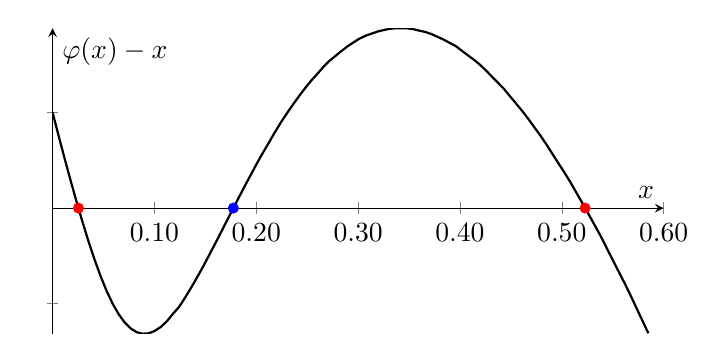
\begin{tikzpicture}[scale=1.0]

\begin{axis}
[
  title={},
  width  = 0.8*0.8*\columnwidth,
  height = 0.8*0.4*\columnwidth,
  axis lines=center,
  legend style={at={(0.95,0.95)}, anchor=north east},
%   xmode=log,
  xlabel={$x$},
  ylabel={$\varphi(x)-x$}, ylabel style={rotate=0},
%  yticklabel=\pgfmathprintnumber{\tick}\\ \%,
  xmin = 0.0, 	
  xmax = 0.6,
%   ymin = -0.05,
%   ymax = 0.05,
  scaled y ticks = false,
  yticklabels={,,},
%   y tick label style={
%         /pgf/number format/.cd,
%         fixed,
%         fixed zerofill,
%         precision=2,
%         /tikz/.cd
%   },
  x tick label style={
        /pgf/number format/.cd,
        fixed,
        fixed zerofill,
        precision=2,
        /tikz/.cd
  },
%   grid = both,
  scale only axis,
]
	\legend{}
    
    \def\k{0.012}
    \def\p{0.100}
    \foreach \a in {0.002}
        \addplot[thick, domain = 0:0.585, samples=100] {(\k*(\a/\p)-\p*x*(\a/\p)^(\k/(\p*x)))/(\k-\p*x)-x};
    
    \fill[color = red]  (axis cs: 0.02539, 0) circle[radius=2pt];
    \fill[color = blue] (axis cs: 0.17750, 0) circle[radius=2pt];
    \fill[color = red]  (axis cs: 0.52286, 0) circle[radius=2pt];
    
    % \foreach \a in {0.1,0.2,0.3,0.4,0.5,0.555,0.62}
    %     \addplot[domain = 0:1, samples=100] {(k*(a/p)-p*x*(a/p)^(k/(p*x)))/(k-p*x)-x};
    
    % \addplot[domain = 0.5:1.04, dashed, samples=100] {x*(1+((-3 + 2*x + sqrt(5 + 4*(-1 + x)*x))/(2*x))*x)*exp(-(2-((-3 + 2*x + sqrt(5 + 4*(-1 + x)*x))/(2*x)))*x)};
    
%     \addplot[thick] table
%     [
% 		x expr = \thisrow{lam},
%     	y expr = \thisrow{25dB}
%     ] {./Data/envelopes.dat};

    % \draw[-\arrowhead] (axis cs: 0.8,0.08) -- (axis cs: 2.7,0.27) node[anchor=south west] 
    %     {$\alpha = 0.1,0.2,0.3,0.4,0.5,0.56,0.62$};
\end{axis}

\end{tikzpicture}

        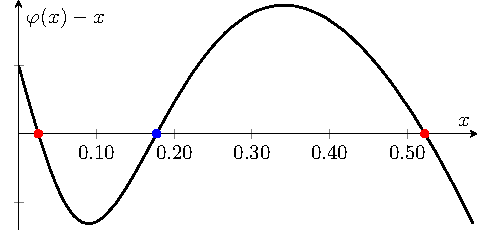
\includegraphics[]{Figures/Ch8_fixed_point.pdf}
    \else
        
\includegraphics[draft,width=\textwidth]{Figures/placeholder.png}
    \fi
    % \includegraphics[width=\columnwidth]{Figures/main-figure0.eps}
    \caption{Red dots are the \textit{attractors} and the blue point is the \textit{repeller}.}
    \label{fig:fixed_point}
\end{figure}

We show in Fig.~\ref{fig:fixed_point} the \textit{attractors} and \textit{repellers}
% \footnote{
% We define \textit{attractor} as a fixed point $x_a$ of $\varphi$ that satisfies $\varphi^n(x)\to x_a$ as $n\to\infty$ for all $x$ in some neighborhood $V_a$ of $x_a$, where $\varphi^n$ denotes repeated composition of the function with itself.
% %
% This neighborhood $V_a$ is called \textit{basin of attraction}.
% %
% A fixed point $x_r$ of $\varphi$ is a \textit{repeller} if there exist $n_0\in\N$ and a neighborhood $V_r$ of $x_r$ such that $\varphi^n(x)\notin V_r$ for all $n > n_0, x\in V_r\backslash\{x_r\}$.
% }
of the chosen scenario, which can be intuitively seen as ``stable'' and ``unstable'' equilibrium points, respectively.
%
The formal definition follows.

\begin{definition}
    A fixed point $x_0$ of a function $\varphi$ is an \textit{attractor} if for all $x$ in some \textit{neighbourhood}\footnote{\textit{Neighborhood} is defined in Definition~\ref{def:neighborhood}.} of $x_0$ we have that $\varphi^n(x) \to x_0$ as $n\to\infty$, where $\varphi^n(x)\triangleq \varphi^{n-1}(\varphi(x))$.
    %
    A \textit{neighbourhood} that satisfies the aforementioned property is a \textit{basin of attraction} for $x_0$.
    
    On the other hand, $x_0$ is a \textit{repeller} if there exists a \textit{neighbourhood} $V$ of $x_0$ and an integer $n_0$ such that for all $x\in V\backslash\{x_0\}$ we have that $\varphi^n(x) \notin V$ for all $n > n_0$.
\end{definition}

\begin{figure}[H]
    \centering
    \if\printfig1
        % 
\begin{tikzpicture}[scale=1.0]

\begin{axis}
[
  title={},
  width  = 0.8*0.8*\columnwidth, 
  height = 0.8*0.5*\columnwidth,
%   axis lines=center,
  legend style={at={(0.95,0.95)}, anchor=north east},
%   xmode=log,
  xlabel={Time slot $t$},
  ylabel={$\bar\rho$}, ylabel style={rotate=-90},
%  yticklabel=\pgfmathprintnumber{\tick}\\ \%,
  xmin = 0, 	
  xmax = 5000,
  ymin = 0.0,
  ymax = 0.65,
  x tick label style={
        /pgf/number format/.cd,
        fixed,
        fixed zerofill,
        precision=0,
        set thousands separator={},
        /tikz/.cd
  },
  grid = both,
  scale only axis,
]
	\legend{}
    
    % \foreach \a in {0.1,0.2,0.3,0.4,0.5,0.555,0.62}
    %     \addplot[domain = 0:1, samples=100] {(k*(a/p)-p*x*(a/p)^(k/(p*x)))/(k-p*x)-x};
    
    % \addplot[domain = 0.5:1.04, dashed, samples=100] {x*(1+((-3 + 2*x + sqrt(5 + 4*(-1 + x)*x))/(2*x))*x)*exp(-(2-((-3 + 2*x + sqrt(5 + 4*(-1 + x)*x))/(2*x)))*x)};

    \addplot[blue!50!black, each nth point=5] table
    [
		x expr = \thisrow{t},
    	y expr = \thisrow{rho1}
    ] {./Data/sim_fixed_point.dat};

    \addplot[green!70!black, each nth point=5] table
    [
		x expr = \thisrow{t},
    	y expr = \thisrow{rho2}
    ] {./Data/sim_fixed_point.dat};
    
    \addplot[brown, each nth point=5] table
    [
		x expr = \thisrow{t},
    	y expr = \thisrow{rho3}
    ] {./Data/sim_fixed_point.dat};
    
    \addplot[magenta, each nth point=5] table
    [
		x expr = \thisrow{t},
    	y expr = \thisrow{rho4}
    ] {./Data/sim_fixed_point.dat};

    \addplot[red,  line width=1.5pt, domain = 0:5000, samples=2] {0.02539};
    \addplot[red,  line width=1.5pt, domain = 0:5000, samples=2] {0.52286};
    \addplot[blue, line width=1.5pt, domain = 0:5000, samples=2] {0.17750};

    % \draw[-\arrowhead] (axis cs: 0.8,0.08) -- (axis cs: 2.7,0.27) node[anchor=south west] 
    %     {$\alpha = 0.1,0.2,0.3,0.4,0.5,0.56,0.62$};
\end{axis}

\end{tikzpicture}
%
        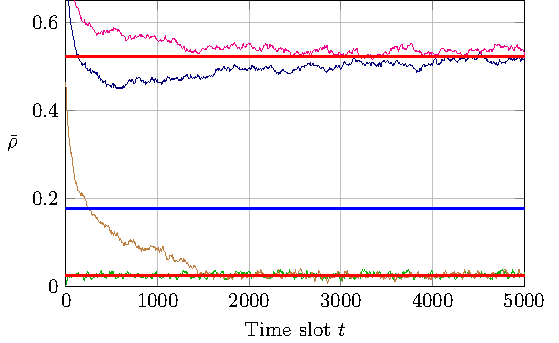
\includegraphics[]{Figures/Ch8_sim_fixed_point.pdf}
    \else
        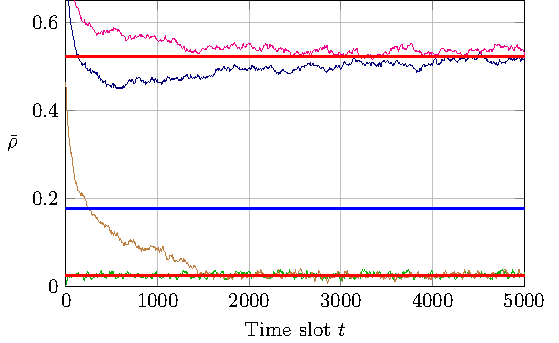
\includegraphics[draft]{Figures/Ch8_sim_fixed_point.pdf}
    \fi
    % 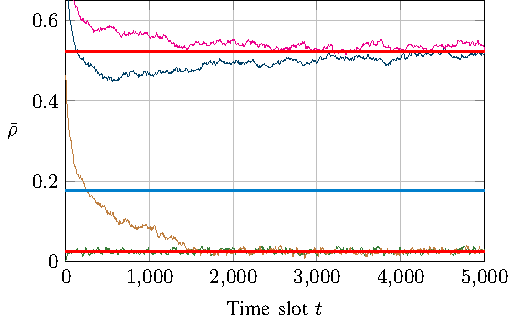
\includegraphics[width=0.8\columnwidth]{Figures/Ch8_sim_fixed_point.eps}
    % \includegraphics[]{Figures/main-figure1.eps}
    \caption{System simulation with four different initial conditions for the queues.
    %
    We show the average proportion of nonempty queues as an estimation of the value of $\bar\rho$.
    %
    The horizontal red lines are the \textit{attractors} and the blue line is the \textit{repeller}.}
    \label{fig:sim_fixed_point}
\end{figure}

Fig.~\ref{fig:sim_fixed_point} shows some simulations, which converge for both \textit{attractors} depending on the initial conditions of the queues. For example, we notice that when queues start heavily loaded, the probability to converge to the upper fixed point increases.
%
The brown curve illustrates that even when we start with initial conditions above the \textit{repeller}, the system may still surpass it.
%
This is due to the fact that the initial conditions do not depend only on the initial mean queue load of the system but also on the number of packets on each one of the queues.
%
In addition, there is ``noise'' in the curves, because we are using a finite number of queues in the simulation, and it tends to vanish as the number of queues tends to infinity.

It is clear that the difference in performance from the upper fixed point to the lower fixed point is immense, e.g., the proportion of unstable queues in one case is $\varepsilon \approx 0.407$, and in the other it is $\varepsilon \approx 9\cdot 10^{-9}$.
%
Thus, when multiple limiting stationary distributions exist, it is then of key importance to operate in the smallest fixed point.

\begin{figure}[htb]
    \centering
    \if\printfig1
        % 
\begin{tikzpicture}[scale=1.0]

\begin{axis}
[
  title={},
%   width  = 0.8*\columnwidth, 
%   height = 0.6*\columnwidth,
%   axis lines=center,
  legend style={at={(0.95,0.95)}, anchor=north east},
%   xmode=log,
  xlabel={$p$},
  ylabel={$\bar\rho$}, ylabel style={rotate=-90},
%  yticklabel=\pgfmathprintnumber{\tick}\\ \%,
%   xmin = 0, 	
  xmax = 1,
%   ymin = 0,
  ymax = 1,
%   x tick label style={
%         /pgf/number format/.cd,
%         fixed,
%         fixed zerofill,
%         precision=2,
%         /tikz/.cd
%   },
  grid = both,
  scale only axis,
]
	\legend{}
    
    % \foreach \a in {0.1,0.2,0.3,0.4,0.5,0.555,0.62}
    %     \addplot[domain = 0:1, samples=100] {(k*(a/p)-p*x*(a/p)^(k/(p*x)))/(k-p*x)-x};
    
    % \addplot[domain = 0.5:1.04, dashed, samples=100] {x*(1+((-3 + 2*x + sqrt(5 + 4*(-1 + x)*x))/(2*x))*x)*exp(-(2-((-3 + 2*x + sqrt(5 + 4*(-1 + x)*x))/(2*x)))*x)};

    \addplot[thick] table
    [
		x expr = \thisrow{p},
    	y expr = \thisrow{rhoL}
    ] {./Data/rhoL_rhoH.dat};

    \addplot[thick, restrict x to domain = 0.083:1] table
    [
		x expr = \thisrow{p},
    	y expr = \thisrow{rhoH}
    ] {./Data/rhoL_rhoH.dat};
    
    \addplot[dashed, restrict x to domain = 0.083:1] table
    [
		x expr = \thisrow{p},
    	y expr = \thisrow{rhoM}
    ] {./Data/rhoL_rhoH.dat};
    
    \addplot[only marks, mark = x, mark size = 3pt] table
    [
		x expr = \thisrow{p},
    	y expr = \thisrow{rho}
    ] {./Data/sim_rho.dat};
    
    % \addplot[red,  line width=3pt, domain = 0:4000, samples=2] {0.0446};
    % \addplot[red,  line width=3pt, domain = 0:4000, samples=2] {0.3854};
    % \addplot[blue, line width=2pt, domain = 0:4000, samples=2] {0.2583};

    % \draw[-\arrowhead] (axis cs: 0.8,0.08) -- (axis cs: 2.7,0.27) node[anchor=south west] 
    %     {$\alpha = 0.1,0.2,0.3,0.4,0.5,0.56,0.62$};
\end{axis}

\end{tikzpicture}
%
        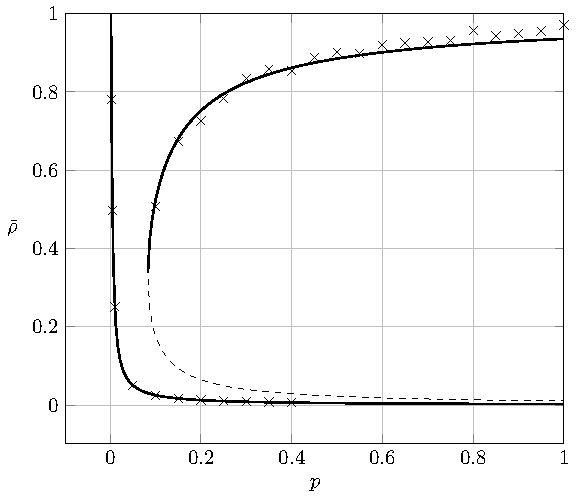
\includegraphics[scale=0.9]{Figures/Ch8_rhoL_rhoH.pdf}
    \else
        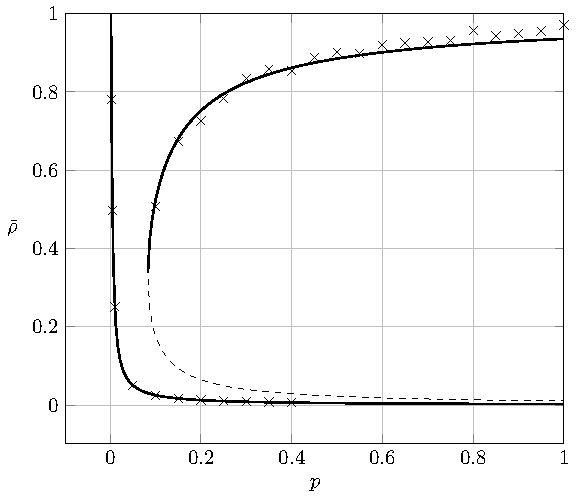
\includegraphics[draft,scale=0.9]{Figures/Ch8_rhoL_rhoH.pdf}
    \fi
    % \includegraphics[width=\columnwidth]{Figures/main-figure2.eps}
    \caption{Solution of $\varphi(\bar\rho)=\bar\rho$ as a function of $p$. The marks are simulation results. The dashed curve is the \textit{repeller} and divides the \textit{basins of attraction}.}
    \label{fig:rhoL_rhoH}
\end{figure}

For that, a simple working strategy is to keep $p$ low, for example $p < \euler\,a$ (which satisfies the uniqueness Theorem~\ref{th:unique_sol2}), until reaching a stationary state, then slowly increase $p$ for all nodes. This would improve the performance (Proposition~\ref{prop:p_opt}) and decrease the probability of converging to another, presumably worse, stationary state.
%
In Fig.~\ref{fig:rhoL_rhoH} we show the theoretical \textit{attractors} and simulate the system using different initial conditions for the queues.
%
Even when employing the strategy of the slowly increasing $p$, we could not make the system converge to the lower fixed point for $p > 0.4$.
%
That was expected at some point, because when $p$ increases, the \textit{basin of attraction} of the lower fixed point becomes smaller and the stochastic nature of the process makes it exit this region and converge to the upper fixed point. %, which has a larger \textit{basin of attraction}.

\begin{note}
    For curiosity, let us present the stationary probability distribution of a queue selected at random from the network system. %
    The equation follows.
    \begin{align*}
        \lim_{t\to\infty}\P\big(Q_0(t) = n\big) &= y \frac{x^y + x^{n+1}(n-y) - x^n (n+1-y)}{(n-y)(n+1-y)}, \quad n\in\N,~ x \triangleq \frac{a}{p}, ~ y \triangleq \frac{\kappa}{p\bar\rho}.
    \end{align*}
    
    Now, the reader may wonder why $Q_0$ does not follow the Geo/Geo/1 distribution at stationary state.
    %
    Indeed, a given queue follows a Geo/Geo/1 at stationary, i.e., $Q_0 \mid R_0$ is a Geo/Geo/1.
    %
    However, before knowing $R_0$ or which queue is selected, we need to take into account the distribution of the queue loads in the network, which results in the cumbersome expression showed above.
    
    Also, note that this distribution is not unique when $\bar\rho$ is not unique.
\end{note}

% % % % % % % % % % % % % % 
\section{Summary} \label{sec:summ_P2_04}

In this chapter, we provided simple sufficient conditions for the uniqueness of a stationary limiting distribution for a Poisson network with general path loss model and general distribution of link distances.
%
The developed mathematical formulation guided us in finding a counterexample to a general uniqueness assumption for the stationary distribution.
%
We verified through extensive simulations that the proposed scenario indeed possesses two very different limiting stationary distributions, which remain valid even when considering a static Poisson network without the main simplifying assumptions of the original system model.

Furthermore, from the uniqueness theorems, we are inclined to conclude (in a more general setting) that this phenomenon of non-unicity is more likely in light traffic scenarios.
%
So those are the cases one must be most wary.
